\documentclass{article}
\usepackage{graphicx} % Required for inserting images
\graphicspath{ {./images/} }
\graphicspath{ {images/} }
\usepackage{xcolor}
\usepackage{amsmath}
\usepackage{multicol}
\usepackage[latin1]{inputenc}
\usepackage[left=1in,right=1in,top=1in,bottom=1in]{geometry}
\usepackage{amsmath}
\usepackage{amsfonts}
\usepackage{amssymb}
\usepackage{url}
\usepackage{hyperref}
\usepackage{mdframed}
\usepackage[hang,flushmargin]{footmisc}
\hypersetup{
    pdftitle={Integral Table from http://integral-table.com},    % title
    pdfauthor={Shapiro},     % author
    pdfsubject={Table of Integrals},   % subject of the document
    pdfcreator={pdftex},   % creator of the document
    pdfproducer={Texmaker}, % producer of the document
    pdfkeywords={CSUN, Integrals, Table of Integrals, Math 280, Math 351, Differential Equations}, % list of keywords
    colorlinks=true,       % false: boxed links; true: colored links
    linkcolor=red,          % color of internal links
    citecolor=red,        % color of links to bibliography
    filecolor=red,      % color of file links
    urlcolor=red           % color of external links
}

\newcommand{\dx}{\hspace{2pt}dx}
\newcommand{\dd}[1]{\hspace{2pt}d#1}
\usepackage{multicol}
\title{Integrals and Applications}
\author{USTH Learning Support}
\date{December 2023}

\begin{document}
\maketitle
\tableofcontents

\pagebreak
\section{Indefinite Integral}

\subsection{Definition:}
An integral \textcolor{blue}{not having any upper and lower limit} is known as an indefinite integral. Mathematically, if F(x) is any anti-derivative of f(x), then the most general antiderivative of f(x) is called an indefinite integral and denoted as:
$$ \int f(x)dx = F(x) + C <=> F'(x) = f(x) $$
\subsection{Properties:}
\\

- A constant factor can be moved through an integral sign:
$$ \int kf(x)dx = k\int f(x) dx = kF(x) + C $$
\\
-An integral of a sum/difference is the sum/difference of integrals:

$$ \int [f(x) \pm g(x)]dx = \int f(x) dx \pm \int g(x) dx = F(x) \pm G(x) + C$$
\\
Here, C is an \textcolor{red}{arbitrary constant}


\begin{center}
\section*{Table of Basic Integrals}

\end{center}

\begin{multicols}{2}

\begin{equation}
\int x^n \dx = \frac{1}{n+1}x^{n+1}, \hspace{1ex} n\neq-1
\end{equation}

\begin{equation}
\int \frac{1}{x}\dx = \ln |x|
\end{equation}

\begin{equation}
\int u \hspace{2pt} \dd{v} = uv - \int v du
\end{equation}

\begin{equation}
\int e^x \dx = e^x 
\end{equation}

\begin{equation}
\int a^x \dx = \frac{1}{\ln a} a^x
\end{equation}

\begin{equation}
\int \ln x \dx = x \ln x - x
\end{equation}


\begin{equation}
\int \sin x \dx = -\cos x
\end{equation}

\begin{equation}
\int \cos x \dx = \sin x
\end{equation}

\begin{equation}
\int \tan x \dx = \ln |\sec x| 
\end{equation}

\begin{equation}
\int \sec x \dx = \ln |\sec x + \tan x|
\end{equation}

\begin{equation}
\int \sec^2 x \dx = \tan x
\end{equation}

\begin{equation}
\int \sec x \tan x \dx = \sec x
\end{equation}

\begin{equation}
\int \frac{a}{a^2+x^2}\dx = \tan^{-1}\frac{x}{a}
\end{equation}

\begin{equation}
\int \frac{a}{a^2-x^2}\dx = \frac{1}{2}\ln\left|\frac{x+a}{x-a}\right|
\end{equation}

\end{multicols}

\subsection{Example:}

Evaluate the following indefinite integrals:
\\
a) \begin{math}
\ \int \frac{1}{2} a^2 da
\end{math}
\\
\\
b) \begin{math}
\ \int \tan(x) dx
\end{math}
\\
\\
\underline{Solution:}
\\
\\
a)
$$ \int \frac{1}{2} \cdot a^2 da = \frac{1}{2} \int a^2 da = \frac{1}{2} . \frac{1}{3} . a^3 + C = \frac{a^3}{6} + C
$$
\\
b) $$
\ \int \tan(x) dx = \int \frac{\sin(x)}{\cos(x)} dx = I
$$
\\
Let $u = \cos(x) => du = -\sin(x)dx$
\\
\\
$$
\ I = \int \frac{\sin(x)}{\cos(x)} dx = \int -\frac{1}{u} du = -\ln|u| + C = -\ln|\cos(x)| + C
$$
\\
\\
You may get the result of $ln|\sec(x)|$ and both are correct:
\\
\\
$$
\ I = -\ln|\cos(x)| + C = 0 - \ln|\cos(x)| + C = \ln|1| - \ln|\cos(x)| + C = ln|\frac{1}{\cos(x)}| + C = ln|\sec(x)| + C
$$
\\
\\
In conclusion:
\begin{mdframed}
$$\ \int \tan(x) dx = -\ln|\cos(x)| + C = \ln|\sec(x)| + C$$
\end{mdframed}

\section{Definition and Properties of Definite Integral}
\subsection{Riemann Sum}
(This is a rather difficult problem. Therefore, if you wish to aim for high grade, you can scroll down to the Appendices section for further details regarding this topic)

\subsection{Properties of definite integrals}
Let f(x) and g(x) be integrable function on the interval [a, b], c and d are constants. Then
\begin{enumerate}
  \item $\int_{a}^{a} f(x) dx = 0 $
  \item $\int_{a}^{b} f(x) dx = -\int_{b}^{a} f(x) dx $
  \item $\int_{a}^{b} c dx = c(b-a) $
  \item $\int_{a}^{b} [cf(x) \pm dg(x)] dx = c\int_{a}^{b}f(x)dx \pm d\int_{a}^{b}g(x)dx $
  \item $\int_{a}^{b} f(x) dx = \int_{a}^{c} f(x) dx + \int_{b}^{c} f(x) dx $
\end{enumerate}

\begin{center}
    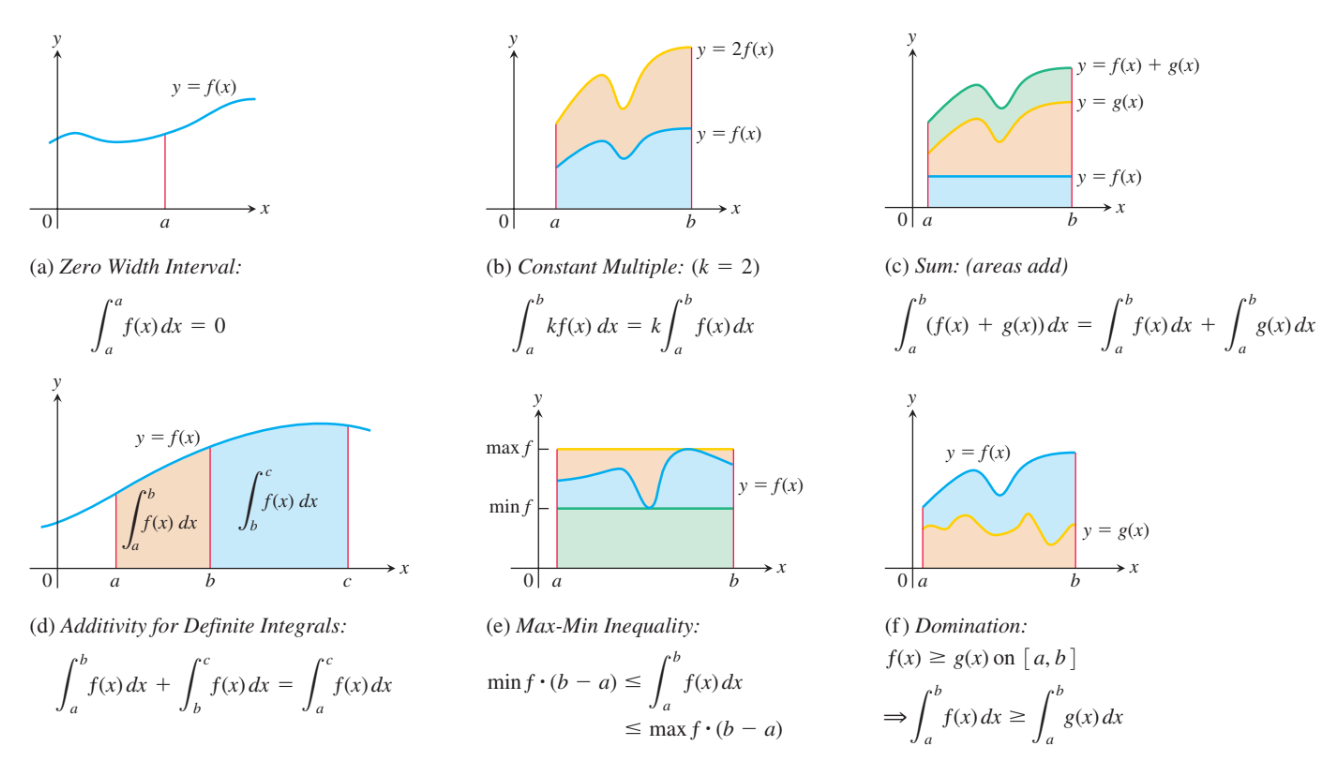
\includegraphics[scale = 0.7]{properties.png}
\end{center}

\subsection{Mean Value Theorem}
If f is continuous on [a, b], then there exists some point c $\in$ [a, b] such that:

$$ f(c) = \frac{1}{b-a} \int_{a}^{b}f(x)dx$$

\begin{center}
    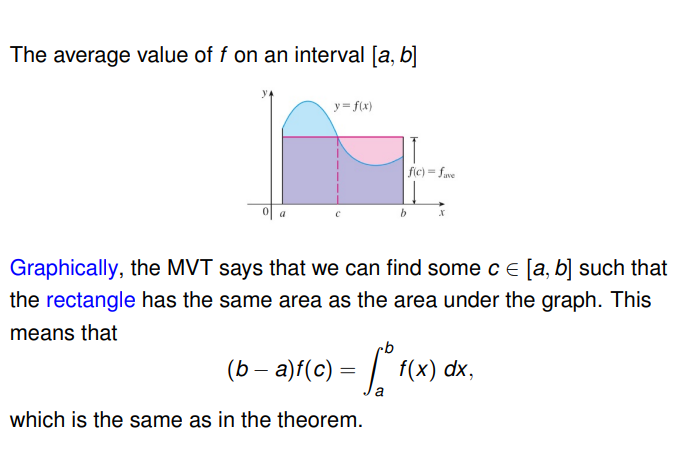
\includegraphics[scale=1]{mvt.png}
\end{center}

\subsection{Example:}

Example 1: Given: $f(x) = 2x + 3$ and $g(x) = x^2 - 1$, integrate $2f(x) + g(x)$ from $a = 0$ to $b = 2$.
\\
\textbf{Step-by-Step Calculation:}

\[
\int_0^2 [2 \cdot (2x + 3) + (x^2 - 1)] \,dx = 2 \cdot \int_0^2 (2x + 3) \,dx + \int_0^2 (x^2 - 1) \,dx
\]

\[
\int_0^2 [2 \cdot (2x + 3) + (x^2 - 1)] \,dx = 2 \cdot \left[\int_0^2 2x \,dx + \int_0^2 3 \,dx\right] + \left[\int_0^2 x^2 \,dx - \int_0^2 1 \,dx\right]
\]

\[
= 2 \cdot \left[x^2 \bigg|_0^2 + 3x \bigg|_0^2\right] + \left[\frac{x^3}{3} \bigg|_0^2 - x \bigg|_0^2\right]
\]

\[
= 2 \cdot [(2^2 + 3 \cdot 2) - (0^2 + 3 \cdot 0)] + \left[\frac{2^3}{3} - 2 - \left(\frac{0^3}{3} - 0\right)\right]
\]

\[
= 2 \cdot (4 + 6) + \left[\frac{8}{3} - 2 - 0\right] = 20 + \frac{8}{3} - 2 = \frac{62}{3}
\]

So, $\int_0^2 [2 \cdot (2x + 3) + (x^2 - 1)] \,dx = \frac{62}{3}$.
\\
\\
Example 2: Given: $c = 4$, $a = 1$, and $b = 3$. Find $\int_a^b c \,dx$.
\[
\int_1^3 4 \,dx = 4 \cdot \int_1^3 1 \,dx = 4 \cdot [x] \bigg|_1^3 = 4 \cdot ( 2 - 1 ) = 8
\]

So, $\int_1^3 4 \,dx = 8$.
\\
\\
Example 3: Given: $\int_1^3 f(x) dx = 2 $ and $\int_3^7 f(x) dx = 8 $. Find $\int_1^7 f(x) dx$

\[
\int_1^7 fx \,dx = \int_1^3 fx \,dx  + \int_3^7 fx \,dx= 2 + 8 = 10
\]

\section{Fundamental Theorems of Calculus}
\subsection{FTC-1}
Suppose that f is continuous on [a, b], and define the function:
\\
\begin{mdframed}
$F(x) = \int_{a}^{x} f(t) dt$ then $F'(x) = f(x)$ for any x of (a,b)
\\
\\
Or usually written in the form:
\\
\\
$$\frac{d}{dx} \int_{a}^{x}f(t)dt = (\int_{a}^{x}f(t)dt)' = f(x)$$
\end{mdframed}
It is important that all three occurrences of the variable x are \textcolor{blue}{consistent}. To apply the FTC-1, the lower limit a must be a constant. If it is not a constant, we must split the integral so that we end up with a constant. In applying the FTC-1, the value of the constant a is \textcolor{blue}{irrelevant}.

\subsection{FTC-2}
If F is an anti-derivative of a continuous function f, then
\begin{mdframed}
    $\int_{a}^{b}f(x)dx = F(b) - F(a) = F(x) \bigg|_a^b $
\end{mdframed}
The FTC-2 is very powerful. It tells us that to compute the value of the definite integral, we do not need to find and use the Riemann sums.Instead, we only need to find some function F with F'(x) = f(x) and calculate F(b) - F(a).

\subsection{Example:}
Example 1: Find
\\
a) $$\frac{d}{dx} \int_0^{x^2}f(t)dt$$
\\
b) $$\frac{d}{d\sqrt{x}} \int_0^{x}f(t)dt$$
\\
Solution:
\\
a) 
Let $y = x^2$ $=> \frac{dy}{dx} = 2x$
\\
We get: $$\frac{d}{dx} \int_0^{x^2}f(t)dt = (\frac{d}{dy} \int_0^{y}f(t)dt) \cdot \frac{dy}{dx} = f(y) \cdot 2x = 2xf(x^2)$$
\\
\\
b)
Let $z = \sqrt{x}$
\\
We get: $$\frac{d}{d\sqrt{x}} \int_0^{x}f(t)dt = \frac{d}{dz} \int_0^{z^2}f(t)dt$$
\\
It's now similar to part a), we put $y = z^2$ $=> \frac{dy}{dz} = 2z $
\\
Then we get: $$\frac{d}{dz} \int_0^{z^2}f(t)dt = (\frac{d}{dy} \int_0^{y}f(t)dt) \cdot \frac{dy}{dz} = f(z^2) \cdot 2z = 2\sqrt{x}f(x)$$

\section{Volumes}
\subsection{Introduction}
In calculus, we can compute volumes of solids of revolution by using integration methods, namely the cross-section and shell methods. These techniques allow us to find the volume of three-dimensional objects formed by rotating a curve around a specific axis.

\subsection{Cross-Section Method}
The cross-section method involves slicing the solid into thin cross-sectional slices perpendicular to the axis of revolution. Consider a solid formed by rotating a curve $y = f(x)$ around the $x$-axis between $x = a$ and $x = b$. Each thin slice at a distance $x$ from the axis has a cross-sectional area $A(x)$. The volume of the solid can be expressed as:

\[
V = \int_{a}^{b} A(x) \, dx
\]

where $A(x)$ represents the area of the cross-section at $x$. For example, if the cross-sections are circles with radius $f(x)$, then $A(x) = \pi [f(x)]^2$.

\subsection{Shell Method}
The shell method involves considering thin cylindrical shells stacked together to form the solid. If the curve $y = f(x)$ is rotated around the $x$-axis between $x = a$ and $x = b$, the volume can be calculated as:

\[
V = \int_{a}^{b} 2\pi x \cdot h(x) \, dx
\]

where $h(x)$ represents the height of the shell at $x$. This method is applicable when the cylindrical shells are perpendicular to the axis of rotation.

\subsection{Example Calculation}
Let's find the volume of the solid obtained by rotating $y = x^2$ around the $x$-axis between $x = 0$ and $x = 2$ using both methods.

{Cross-Section Method}
For the cross-section method, each slice at $x$ has an area $A(x) = \pi [f(x)]^2 = \pi x^4$. Therefore,

\[
V = \int_{0}^{2} \pi x^4 \, dx
\]

{Shell Method}
Using the shell method, we take r = y as the radius for the base. Then, the height $y$ is $h(y) = 2 - \sqrt{y}$. The radius y runs from 0 to 4. Thus

\[
V = \int_{0}^{4} 2\pi y \cdot (2-\sqrt{y}) \, dy
\]
\begin{center}
    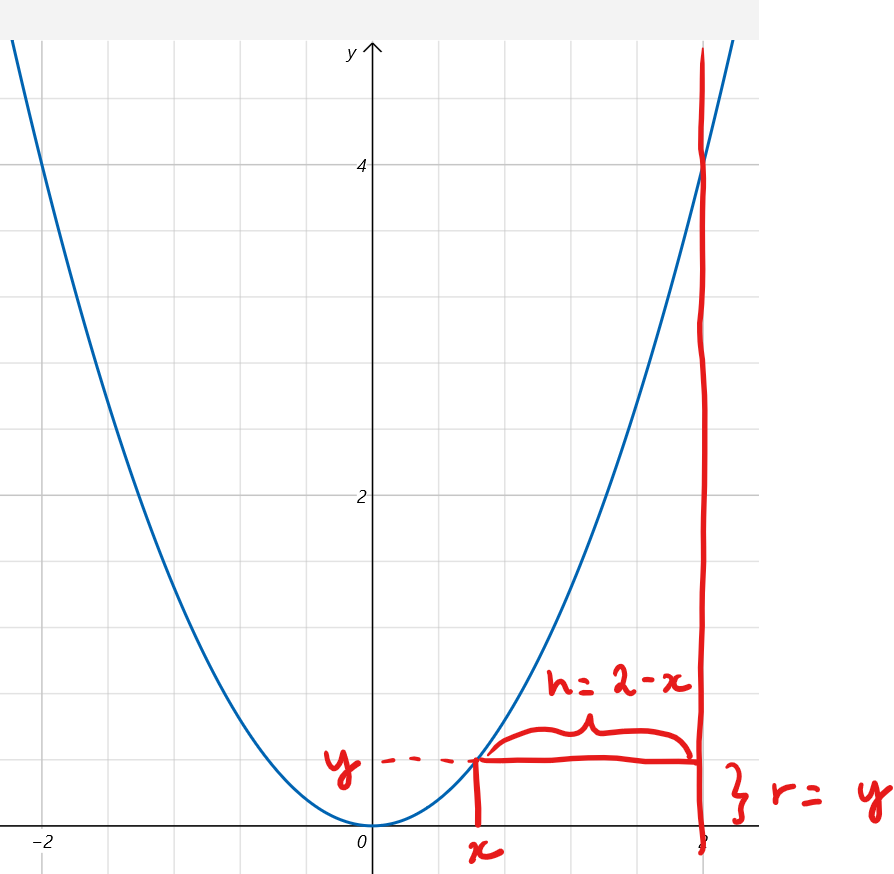
\includegraphics[scale = 0.7]{shell.png}
\end{center}
Solving these integrals will give us the volume of the solid using both methods.
\pagebreak
\\
Let's consider another example:
The region bounded by the curve y = $\sqrt{x}$, the x-axis, and the line x = 4 is revolved about the x-axis to generate a solid. Find the volume of the solid by the \textcolor{blue}{shell method}.
\begin{center}
    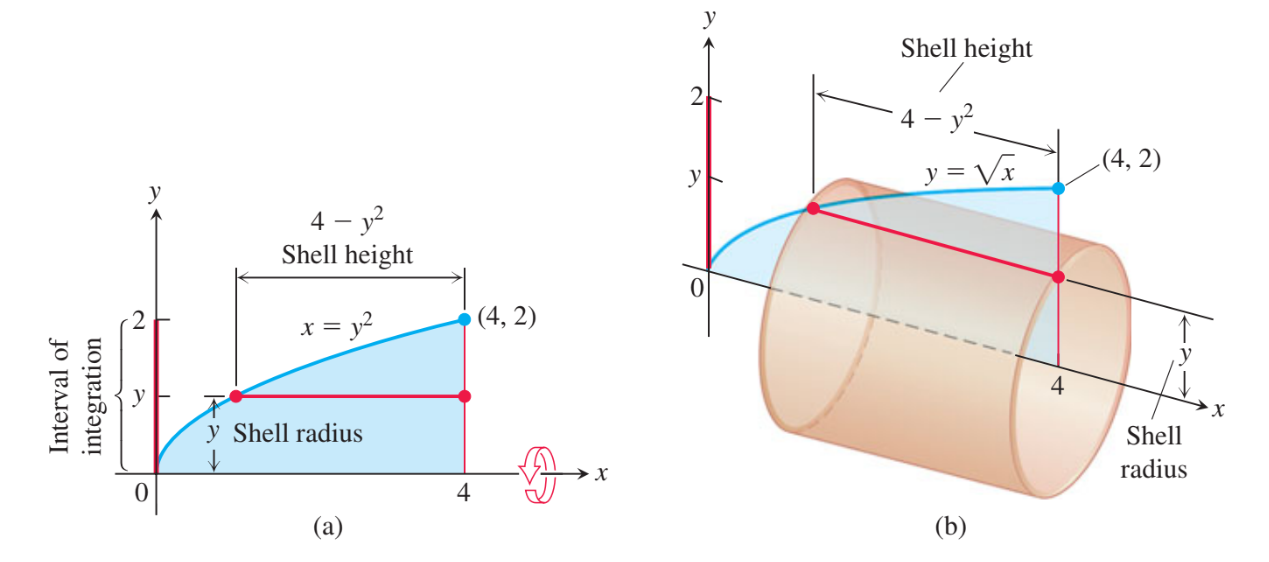
\includegraphics[scale = 0.35]{image_2023-12-18_215922175.png}
\end{center}
In this case, the shell thickness variable is y, so the limits of integration for the shell formula method are $a = 0$ and $b = 2$ (along the y-axis in the figure above). The volume of the solid is
\begin{align}
    V &= 2\pi \int_{a}^{b} \text{shell radius}*\text{shell height}*dy\\
    &= 2\pi \int_{0}^{2} (y)*(4-y^2)*dy\\
    &= 2\pi \int_{0}^{2} (4y-y^3)dy\\
    &= 2\pi \left[2y^2-\frac{y^4}{4}\right]_0^2 = 8\pi
\end{align}
\section{Arc Length and Surface Area}
\subsection{Arc Length}
The arc length of a smooth curve $y = f(x)$ between $x = a$ and $x = b$ can be computed using the formula:

\[
L = \int_{a}^{b} \sqrt{1 + \left(\frac{dy}{dx}\right)^2} \, dx
\]

where $\frac{dy}{dx}$ represents the derivative of $f(x)$ with respect to $x$. This integral represents the accumulation of infinitesimal line segments along the curve, resulting in its total length.

\subsection{Surface Area of Revolution}
When a curve $y = f(x)$ is rotated around the $x$-axis between $x = a$ and $x = b$, the surface area $S$ of the resulting surface of revolution can be calculated using integration:

\[
S = 2\pi \int_{a}^{b} f(x) \sqrt{1 + \left(\frac{dy}{dx}\right)^2} \, dx
\]

This formula considers the circumference of the circular cross-sections formed by the curve and sums them up along the curve, integrating to find the total surface area.

\subsection{Example Calculations}
Let's find the arc length and surface area for the curve $y = \ln(x)$ between $x = 1$ and $x = e$.

\subsubsection{Arc Length}
For the arc length, we compute:

\[
L = \int_{1}^{e} \sqrt{1 + \left(\frac{d}{dx}(\ln(x))\right)^2} \, dx
\]

\subsubsection{Surface Area of Revolution}
For the surface area, rotating $y = \ln(x)$ around the $x$-axis:

\[
S = 2\pi \int_{1}^{e} \ln(x) \sqrt{1 + \left(\frac{d}{dx}(\ln(x))\right)^2} \, dx
\]

\begin{center}
    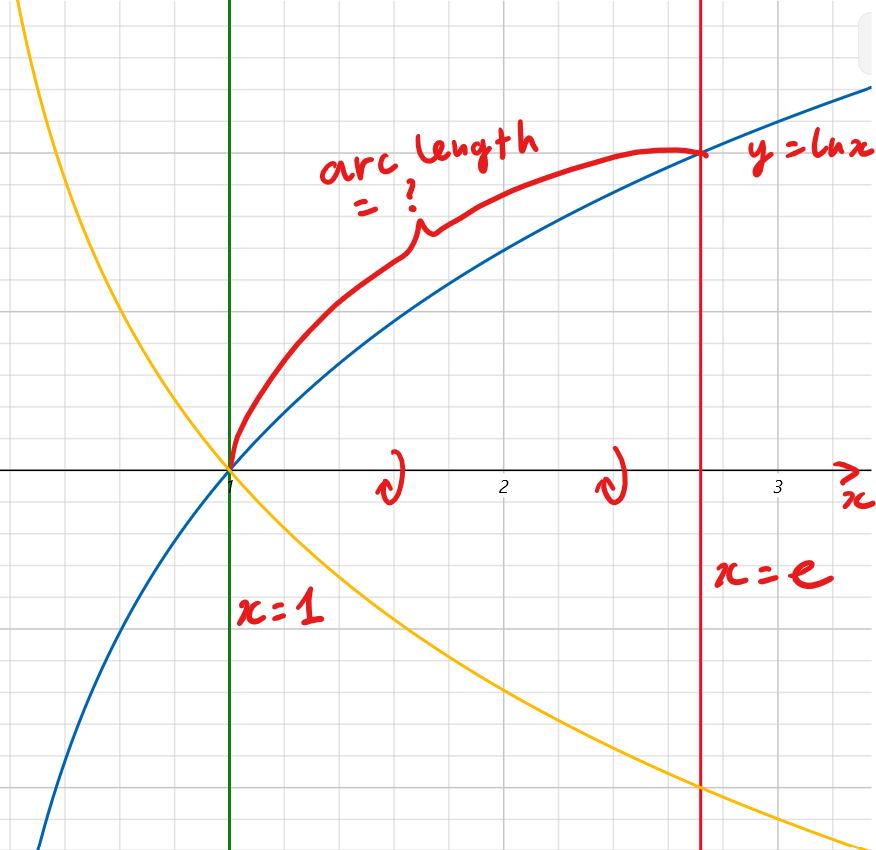
\includegraphics[scale = 0.5]{arc.png}
\end{center}
Solving these integrals will give us the arc length and surface area for the specified curve.

\section{Appendix: Riemann Sums}
\subsection{Definition}
Riemann sums approximate the area under the curve by dividing the interval $[a, b]$ into $n$ subintervals and summing the areas of rectangles.

The width of each subinterval $\Delta x$ is given by $\frac{b - a}{n}$.

The height of each rectangle is taken as the value of the function at some point within the subinterval. We can use the left, middle or right endpoints of each subinterval.

The Riemann sum can be written as:
\[ \frac{b-a}{n}\sum_{i=1}^{n} f(x_i^*) \]
where the points $a = x_0 < x_1 < ... < x_{n-1} < x_n = b$ divide up the interval [a, b] into n equal subintervals, and $x^{*}_{i} \in [x_{i-1}, x_{i}]$ are sampling points.
Note that as a sampling point, it is most commonly to take:
\begin{enumerate}
    \item the left-endpoint $x^*_i = x_{i-1}$, or
    \item the the right-endpoint $x^*_i = x_i$, or
    \item the midpoint $x^*_i = \frac{x_{i-1} + x_i}{2}$
\end{enumerate}

The Riemann integral of the function f(x) from a to b is the
limit of the Riemann sums as n $\to \infty$ . That is

$$ \int_{a}^{b} f(x) dx = \lim_{n \to \infty} \frac{b-a}{n} \sum_{i=1}^{n} f(x_i^*)$$

\begin{center}
    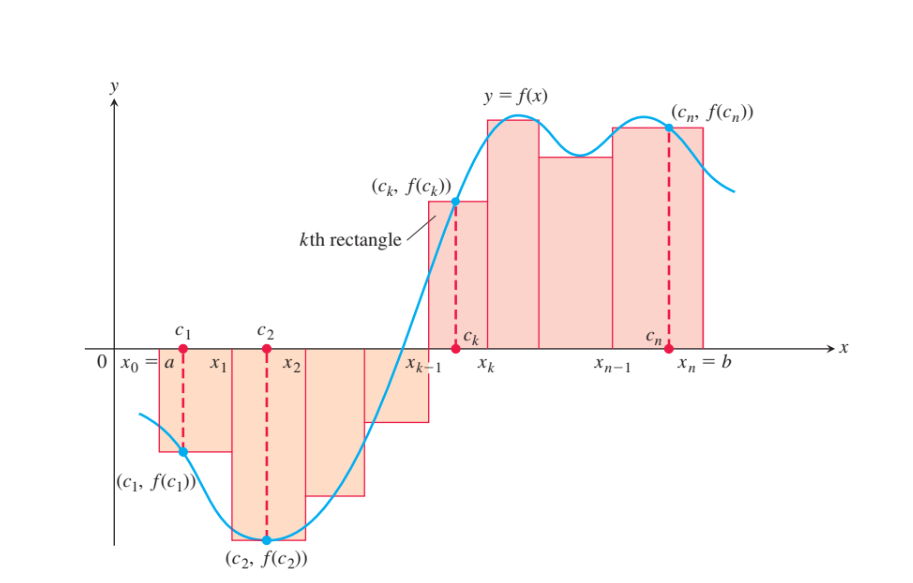
\includegraphics[scale=0.5]{image_2023-12-18_214927179.png}
\end{center}
\pagebreak
There are some basic sums that you need to remember when doing these exercises:
\begin{enumerate}
    \item $$\sum_{i=1}^{n} i = \frac{n \cdot (n+1)}{2}$$
    \item $$\sum_{i=1}^{n} i^2 = \frac{n \cdot (n+1) \cdot(2n+1)}{6}$$
    \item $$\sum_{i=1}^{n} i^3 = \left(\frac{n \cdot (n+1)}{2}\right)^2$$
\end{enumerate}

\subsection{Example:}
Example 1: Use the definition of integral to calculate:
$$\int_{0}^{3} (x^2 + 1) dx$$
Solution:
We divide the interval [0, 3] into n equal subintervals, then:
$x_1 = 0, x_{n+1} = 3$ and $x_i =  \frac{3 \cdot i}{n}$ for $k = 2, . . . n.$
We choose $x^*_i$ to be the right-end points $=> x^*_i = \frac{3i}{n}$
From then, we have:
$$\int_{0}^{3} (x^2 + 1) dx = \lim_{n\to\infty} \frac{3-0}{n} \sum_{i=1}^{n} f(x^*_i) = \lim_{n\to\infty} \frac{3}{n} \sum_{i=1}^{n} ((\frac{3i}{n})^2+1)$$$$ = \lim_{n\to\infty} \frac{3}{n} \cdot \left(\sum_{i=1}^{n} \frac{9i^2}{n^2} + \sum_{i=1}^{n} 1 \right) = \lim_{n\to\infty} \frac{27}{n^3} \sum_{i=1}^{n} i^2 + \lim_{n\to\infty} \frac{3}{n} \sum_{i=1}^{n} 1$$ 
$$ = \lim_{n\to\infty} \frac{27}{n^3} \cdot \frac{n(n+1)(2n+1)}{6}+ \lim_{n\to\infty} \frac{3}{n} \cdot n$$
$$= \lim_{n\to\infty} \cdot \frac{27(1+\frac{1}{n})(2+\frac{1}{n})}{6} + 3 = 9 + 3 = 12$$
\\
Example 2: Use the definition of integral to calculate:
$$\int_{0}^{2} x^3 dx$$
Solution: We divide the interval [0, 2] into n equal subintervals and then choose $x^*_i$ to be right point, $x^*_i = \frac{2i}{n}$. From then, we have:
$$\int_{0}^{2} x^3 dx = \lim_{n\to\infty} \frac{2-0}{n} \sum_{i=1}^{n} f(x^*_i) = \lim_{n\to\infty} \frac{2}{n} \sum_{i=1}^{n} (\frac{2i}{n})^3$$
$$= \lim_{n\to\infty} \frac{16}{n^4} \sum_{i=1}^{n} i^3 = \lim_{n\to\infty} \frac{16}{n^4} \left(\frac{n\cdot(n+1)}{2}\right)^2$$
$$= \lim_{n\to\infty} \frac{4 \cdot n^2\cdot(n+1)^2}{n^4} = \lim_{n\to\infty} 4 \cdot \left(\frac{n+1}{n}\right)^2$$
$$= \lim_{n\to\infty} 4 \cdot \left(1+ \frac{1}{n}\right)^2 = 4 \cdot 1 = 4$$
\end{document}
